\documentclass[letterpaper]{article}

%%% Load packages %%%%%%%%%%%%%%%%%%%%%%%%%%%%%%%%%%%%%%%%%%%%%%%%

\usepackage{fontspec}
%[
%Renderer=Graphite,
%RawFeature={onum}]
\setmainfont{Libertinus Serif}[
Ligatures={Common,TeX},
Numbers={OldStyle, Proportional}
]
\setsansfont{Libertinus Sans}
\setmonofont[Scale=MatchLowercase]{Libertinus Mono}

\usepackage{amsmath}
\usepackage{unicode-math}
\setmathfont[Scale=MatchLowercase]{Libertinus Math}

%% some frequently-used commands
\newcommand{\fslining}[1]{{\addfontfeatures{Numbers=Lining}{#1}}}
\newcommand{\fssup}[1]{{\addfontfeatures{VerticalPosition=Superior}{#1}}}
\newcommand{\fssc}[1]{{\addfontfeatures{Letters=SmallCaps}{#1}}}
%% Language and font encodings
% supersedes babel, http://www.ctan.org/tex-archive/macros/xetex/latex/polyglossia
\usepackage{polyglossia} 
\setdefaultlanguage[]{english}

% \usepackage{tabu}
% \usepackage[T1]{fontenc}

% Setup page size specifically
%\usepackage[twoside,paperheight=240mm,paperwidth=170mm,centering,height=186mm,width=120mm,outermargin=45mm]{geometry}
%\usepackage[xetex,twoside,paperheight=240mm,paperwidth=170mm,centering]{geometry}
\usepackage[letterpaper,xetex,twoside]{geometry}

% Some improvements for xetex and latex. Loads fixltx2e, metalogo, xunicode, fontspec.
% http://mirror.math.ku.edu/tex-archive/macros/latex/contrib/fontspec/fontspec.pdf
% \usepackage[no-math]{fontspec}
% \usepackage{xunicode}

% Load colors with names
\usepackage[usenames]{color}
% For headers 
\usepackage{fancyhdr}

%% Useful packages
\usepackage[font=footnotesize]{caption}
\usepackage{subcaption}
\usepackage{graphicx}
\usepackage{booktabs}
\usepackage[inline]{enumitem}
%\usepackage{apacite}
% \usepackage[colorinlistoftodos]{todonotes}

% For clickable URLS/references/etc. within the PDF document
\usepackage[]{hyperref}
%%% Hyperref setup %%%%%%%%%%%%%%%%%%%%%%%%%%%%%%%%%%%%%%%%%%%%%
\hypersetup{
pdfauthor = {Ali Alizadeh Mansouri},
pdftitle = {Big Data Analytics Project Report},
pdfsubject = {Big Data Analytics Project Report},
pdfkeywords = {Big Data, Fog Computing},
pdfcreator = {XeLaTeX with hyperref package},
pdfproducer = {pdfLaTeX},
colorlinks = true,
breaklinks = true,
linkcolor = red,          % color of internal links
citecolor = magenta,        % color of links to bibliography
filecolor = magenta,      % color of file links
urlcolor = blue,          % color of external links
}

% urls will have the same font and styling as the text (useful for urls in footnotes)
\urlstyle{same}

\def\@cite#1#2{[\fslining{{#1\if@tempswa , #2\fi}]}}

\title{Big Data Analytics Project Proposal\\
        \large A Fog Computing Prototype}

\author{
    Ali Alizadeh Mansouri\\
    \fslining{40102969}
    \and
    Marco Sassano\\
    \fslining{26658245}
    }
\date{}

 %%% commands %%%%%%%%%%%%%%%%%%%%%%%%%%%%%%%%%%%%%%%%%%%%%%%%
\newcommand{\etal}{\emph{et\,al.}\,}
% set the paragraph indent to zero,
% and the paragraph spacing to 0.5\baselineskip
\setlength{\parindent}{0pt}
\setlength{\parskip}{0.5\baselineskip}%

\begin{document}
\maketitle

\begin{abstract}
Internet of Things (IoT) aims to bring every object (e.g. smart cameras, wearables, environmental sensors, home appliances, and vehicles) online, hence generating massive volumes of data that can overwhelm storage systems and data analytics applications. Cloud computing offers services at the infrastructure level that can scale to IoT storage and processing requirements. However, there are two major downsides to this two-layer infrastructure: The bottleneck is the network bandwidth, meaning that transmission of large volumes of raw data will oversaturate the network bandwidth on the way to the cloud, and there will be a high latency and response time for the results to come back from the cloud to the IoT devices. To overcome this limitation, Fog computing paradigm has been proposed, where cloud services are extended to the edge of the network to decrease the latency and network congestion. In our project, we implemented a Fog Computing infrastructure for early detection of epilepsy seizures using EEG timeseries data consisting of three layers: IoT devices and sensors, a Fog layer, and the Cloud. We performed the analytics on the 2\fssup{nd} and the 3\fssup{rd} layers. We report the methods, the results, and discuss the possible challenges, limitations, and future work.
 \end{abstract}

 %%% Introduction %%%%%%%%%%%%%%%%%%%%%%%%%%%%%%%%%%%%%%%%%%%%%%%%
 
 \section{Introduction}\label{introduction}
The number of Internet of Things (IoT) devices has increased to a great extent in recent years. It is estimated that 50 billion devices will be connected to the internet by 2020\,\cite{cisco2011}. On the other end side of the infrastructure, Cloud computing as a paradigm delivers computing services over the internet --- the Cloud --- to offer flexible resources to deal with a wide range of scalable computational demands. This includes analysis, aggregation, and storage of large volumes of data (Big Data) from the IoT devices. The total internet bandwidth crossing international borders in 2013 was 100 Tbps. Furthermore, while application demands are growing from 100s of terabytes towards petabytes per day, network capacity growth has been decelerating\,\cite{GlobalAnalytics2015}. In other words, the bottleneck of such infrastructure lies on the network bandwidth between the IoT devices and the Cloud. This issue arises from the fact that most Cloud computing datacenters are geographically centralized, and situated far from the proximity of the end devices.

Fog Computing (FC) was proposed by Cisco in 2012 to address the needs of the applications which demand low latency and high response times\,\cite{cisco2012}. As a distributed computing paradigm, FC acts as an intermediate layer in between Cloud services and IoT devices (or end users/devices in general)\,\cite{Mahmud2018}. In this manner, the concept of FC is analogous to \emph{data locality}, in which computational tasks are moved towards the data, instead of the other way.
%  Figure \ref{fig-fog-computing} shows a typical FC environment.

% Moreover, FC facilitates location awareness, mobility support, real-time interactions, scalability and interoperability\,\cite{cisco2012}.

% \begin{figure}
%     \label{fig-fog-computing}
%     \centering
%         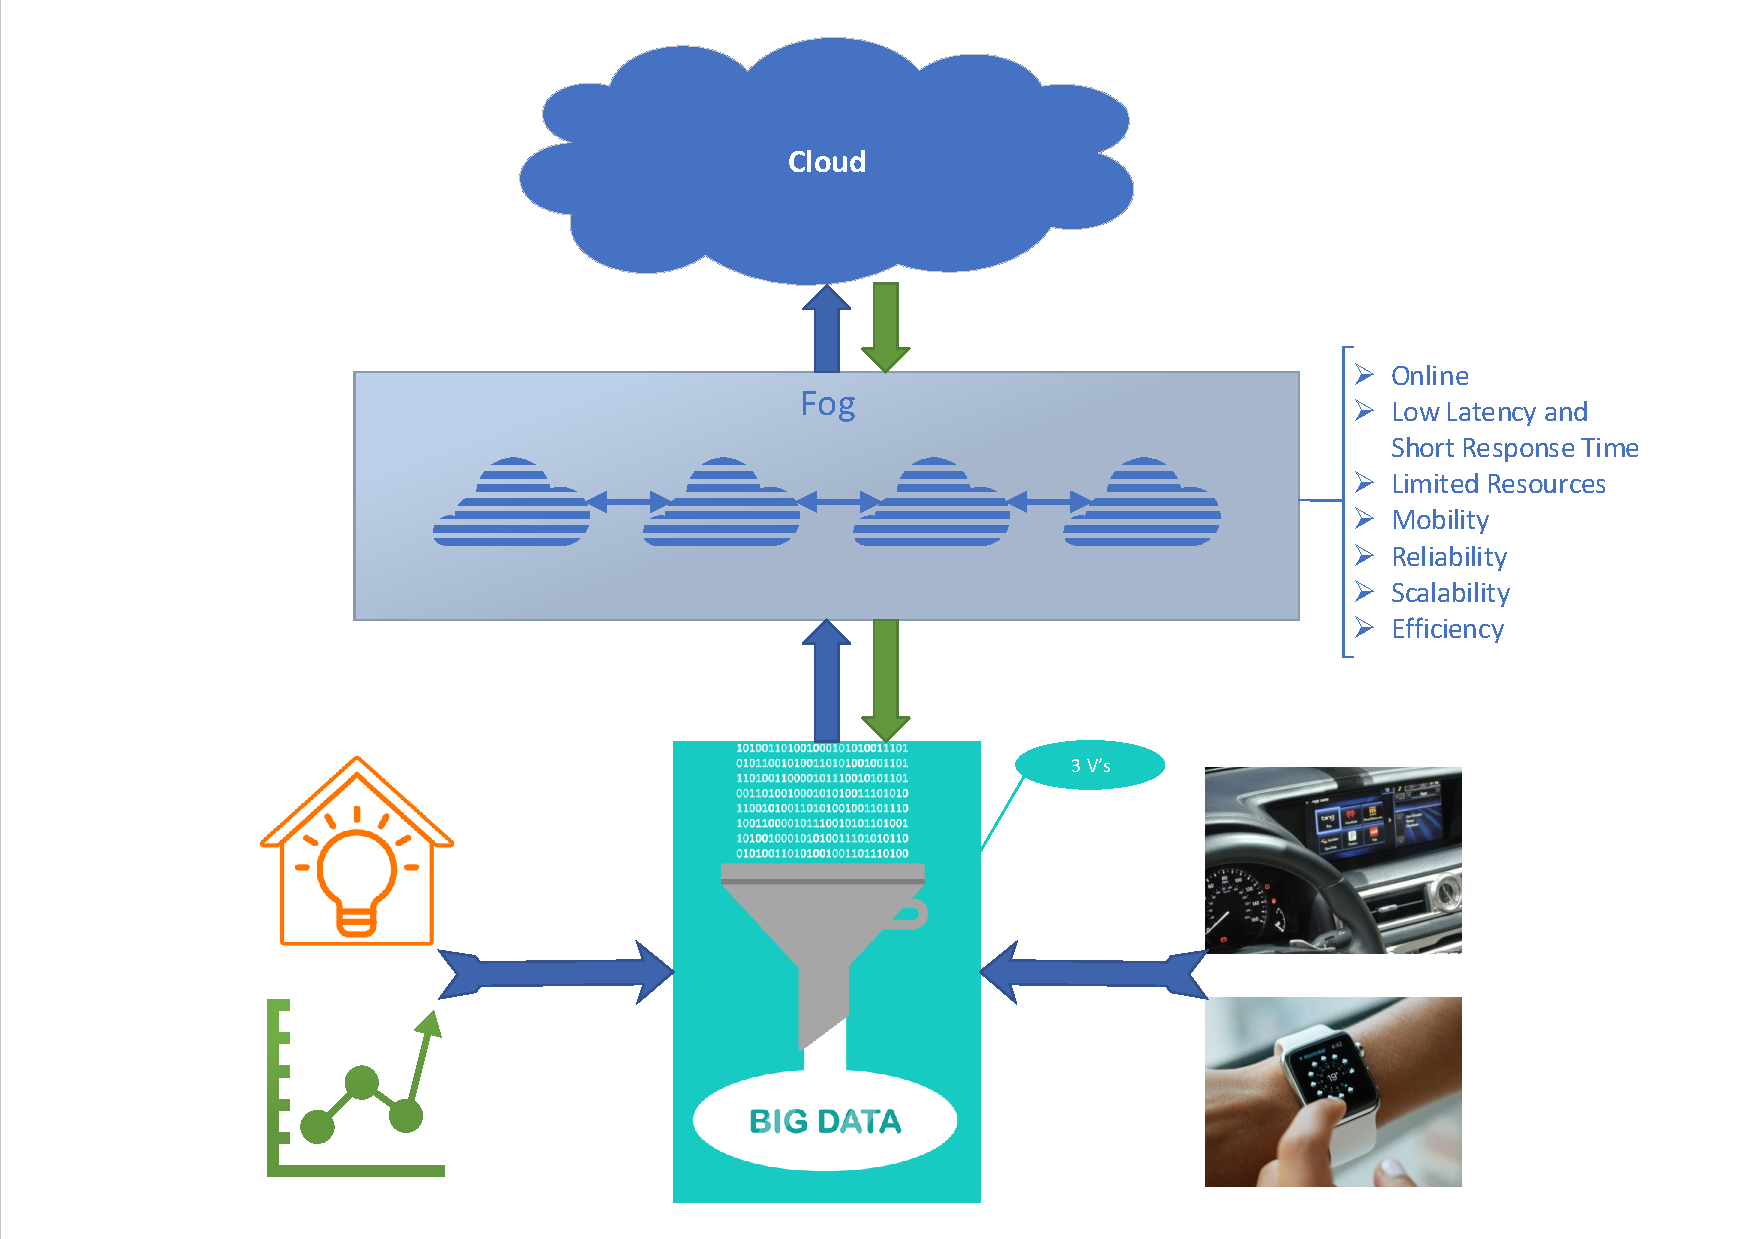
\includegraphics[width=0.4\textwidth]{figs/Data_Stream_Processing_in_Fog_Computing.pdf}
%     \caption{A Fog Computing environment.}
%   \end{figure}

% It is worth mentioning that, FC is sometimes referred to as ``Edge Computing'' in the literature (e.g.\,\cite{Shi2016,GarciaLopez2015}). Certain surveys, on the other hand, treat the two as separate paradigms by considering FC as a generalization of Edge Computing, with Edge Computing representing a set of network devices (including the end devices) not necessarily interacting with the cloud\,\cite{Mahmud2018}. For the sake of clarity, we will use ``FC'' to refer to the paradigm in the focus of this project, as suggested by\,\cite{cisco2012} and\,\cite{Mahmud2018}.

\subsection{Problem Specification}
We consider the healthcare application of early detection of epilepsy seizures using EEG timeseries data, because such healthcare applications require close to real-time response times.

Our goal was to achieve less network congestion between the Fog and Cloud layers as well as higher response times for the EEG sensors. More specifically, we aim for a balanced tradeoff between fast and light-weight --- even though less accurate --- computations on the IoT side, and more accurate classifications but with higher latency on the cloud side.\footnote{\emph{A note on the revision of the first two sections}: Compared to the project proposal, these sections have been mildly revised to \begin{enumerate*}[label=\arabic*)]
    \item more accurately reflect the actual implementation of the project, and the materials --- including the dataset used --- and,
    \item incorporate the professor's helpful comments from the project proposal.
  \end{enumerate*}}

\subsection{Related Work}
FC in general as well as different applications requiring real-time response times have been considered vastly in the literature. For example, Tang \etal\cite{Tang:2015} implemented a hierarchical FC architecture for anomaly detection of pipe leakage in smart cities. We were inspired by the work of Diab Abdulgalil \etal\cite{DiabAbdulgalil2018}, where they propose a FC architecture with SVM classification at the edge, and deep convolutional networks in the cloud. To the best of our knowledge, and to the date of this writing, this has been the only work which considered FC for efficient epilepsy seizures detection.

%%% Materials and Methods %%%%%%%%%%%%%%%%%%%%%%%%%%%%%%%%%%%%%%%%%%%%%%%%

 \section{Materials and Methods}\label{materials}

 \subsection{Dataset}
 Andrzejak \etal\cite{PhysRevE.64.061907}\footnote{\url{http://epileptologie-bonn.de/cms/front_content.php?idcat=193&lang=3&changelang=3}} provide a dataset of \(500\) individuals, each with \(4097\) data points for \(23.5\) seconds. This dataset is further reshaped and shuffled to \(23 \times 500 = 11500\) records, where each record contains \(178\) data points (features) for \(1\) second by Qiuyi and Fokoue on UCI Machine Learning Repository \cite{UCIDataset}. Each record of this dataset is labeled with one of 5 classes, with one class being the seizure state. Since our goal was predicting the seizures, we further restructured this dataset into \texttt{(time,value)} tuples, and considered the seizure class of consecutive \(178\) tuples as positive, and all the groups of tuples belonging to other classes as negative. This resulted in \(11500 \times 178 = 2\,047\,000\) tuples, which would be simulated as a stream of data generated by an EEG sensor. The final breakdown of the dataset is shown in table~\ref{tab.dataset}.

\begin{table}
  \centering
  \caption{The breakdown of the EEG timeseries dataset used. Each record represents 178 tuples in a window of one second.}
  \label{tab.dataset}
  \addfontfeatures{Numbers={Lining,Tabular}}
  {\begin{tabular}{@{} lrrr @{}}
    \toprule
      & Total & Positive & Negative\\
    \midrule
    Training & 7\,000 & 1\,392 & 5\,608\\
    Test & 4\,500& 908 & 3\,592\\
    \addlinespace
    Total & 11\,500 & 2\,300 & 9\,200\\
    \bottomrule
  \end{tabular}}
\end{table}

 \subsection{Project Structure}
 We will consider a three-tier architecture for our FC implementation, as described below:

 \begin{enumerate}
     \item \textbf{The sensor:} This layer consists of the EEG sensor, which generates streams of tuples in the form of \texttt{(time,value)}.       

     \item \textbf{The edge layer:} The edge layer\footnote{It is worth mentioning that, Fog Computing is sometimes referred to as ``Edge Computing'' in the literature (e.g.\,\cite{Shi2016,GarciaLopez2015}). Certain surveys, on the other hand, treat the two as separate paradigms by considering Fog Computing as a generalization of Edge Computing, with Edge Computing representing a set of network devices (including the end devices) not necessarily interacting with the cloud\,\cite{Mahmud2018}. For the sake of clarity, we will use ``Fog Computing'' to refer to the paradigm in the focus of this project, as suggested by\,\cite{cisco2012} and\,\cite{Mahmud2018}.} is the intermediate layer between the sensor and the cloud. Its job is to map and analyze the stream of tuples from the sensor.          

     \item \textbf{The cloud:} The cloud in a conventional FC architecture receives the preliminary results of the edge layer for further analysis and aggregation. However, we perform the analytics on the same dataset in the cloud in order to compare the performance of the two layers more accurately in terms of accuracy and resource consumption.
 \end{enumerate}

 \subsubsection{The Edge}
 At the time of this writing, there are only two frameworks dedicated to Fog/Edge Computing: Apache Edgent\footnote{\url{http://edgent.apache.org/}}, and iFogSim\,\cite{iFogSim}\footnote{\url{https://github.com/Cloudslab/iFogSim}} both of which are currently in a beta state. After an initial inspection, we chose Apache Edgent because it is in active development and more mature.
 
 We implemented the sensor and the edge layers using Apache Edgent, which is a program model and runtime environment in Java suitable for stream processing. The sensor is implemented using a \textbf{Supply} class, whose job is to simulate generation of infinite streams of data from a variety of sources, including files, databases, network/internet resources, and physical sensors. In our case, we read the dataset, and output the tuples as a stream.

The edge layer consists of two parts:
\begin{itemize}
  \item \textbf{Map:} As described previously, our goal was to come up with a fast and light-weight detection algorithm. Carney \etal\cite{Carney2011} compared several epilepsy detection algorithms, from simple aggregation-style statistical measures, to more complicated machine learning algorithms such as deep convolutional networks. We experimented and compared the accuracy of the more simpler methods --- to be more consistent with our goal --- such as standardized moments (variance, skewness, kurtosis). Based on analysis of the dataset, we decided that the root of the sum of squared distances between every consecutive pair of tuples best describes the seizure classes of records. We denote this measure using \(\mathcal{D}\), shown in equation~\ref{eq.Delta}. The \(\mathcal{D}\) measure is implemented in the \emph{map} step, which receives streams of tuples from the sensor, and maps them to \texttt{(\(\mathcal{D}\))} tuples as another stream.
  \begin{equation}
    \label{eq.Delta}
    \mathcal{D} = \sqrt{\sum_{i=2}^{n}{(X_i - X_{i-1})^2}}    
  \end{equation}
  \item \textbf{Analyze:} This step will classify every window of \(178\) tuples (equivalent to one second of data points) according to a threshold \(\Theta\). The threshold \(\Theta\) is the determined optimal value among different \(\mathcal{D}\) candidates obtained from the previous step on the training phase. Any values of \(\mathcal{D} > \Theta\) will be classified and detected as an indication of seizure on the testing phase.
\end{itemize}

Figure~\ref{fig.edge-pipeline} shows the described edge pipeline.

\begin{figure}
  \centering
  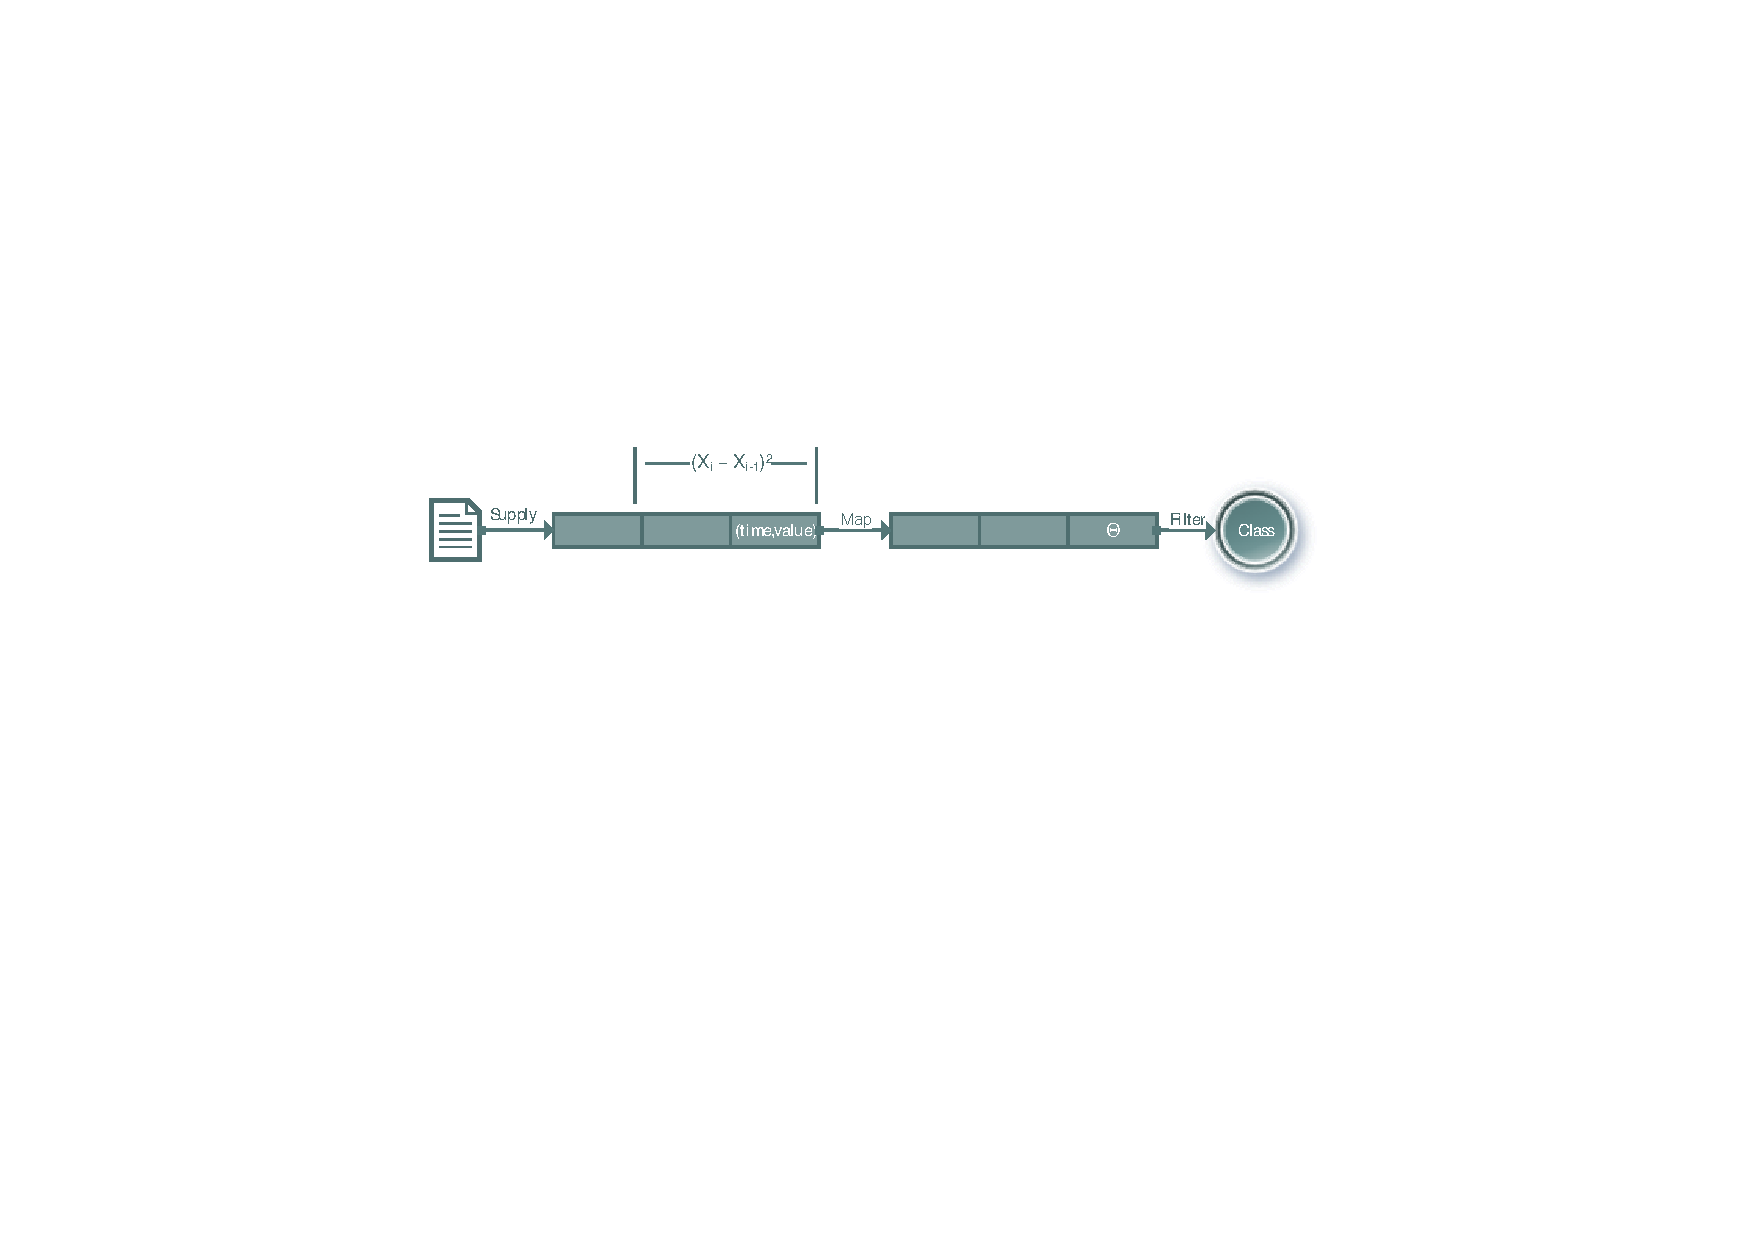
\includegraphics[width=\textwidth]{figs/Edgent_pipeline.pdf}
  \caption{The implemented edge stream processing pipeline.}
  \label{fig.edge-pipeline}
\end{figure}

\subsubsection{The Cloud}

The \emph{k-means} algorithm is mentioned as one of the epilepsy seizure detection methods by Carney \etal\cite{Carney2011}. It is also the major method used for anomaly detection in the \textsc{egads} library by Yahoo~\cite{egads}\footnote{\url{https://github.com/yahoo/egads}}. Therefore, we implemented the cloud analytics step using the \emph{k-means} algorithm, with the number of classes/clusters predetermined in our dataset. We implemented our algorithm using Python on Apache Spark (PySpark) as an efficient parallelized computing framework.

As the measure of distance, we experimented with the Euclidean distance. We also tried transforming data into 178 dimensions. However, we did not achieve a good accuracy due to, what we believe to be, different time intervals present in the dataset. We ultimately selected a distance measure similar to the edge layer, which is the sum of absolute consecutive pairwise differences for each window of 178 tuples, here denoted by \(\mathcal{S}\) and shown in equation~\ref{eq.S}.
\begin{equation}
  \label{eq.S}
  \mathcal{S} = \sum_{i=2}^{n}{\left|X_i - X_{i-1}\right|}
\end{equation}

\section{Results}

\begin{figure*}
  \centering
  \begin{subfigure}[b]{0.475\textwidth}
      \centering
      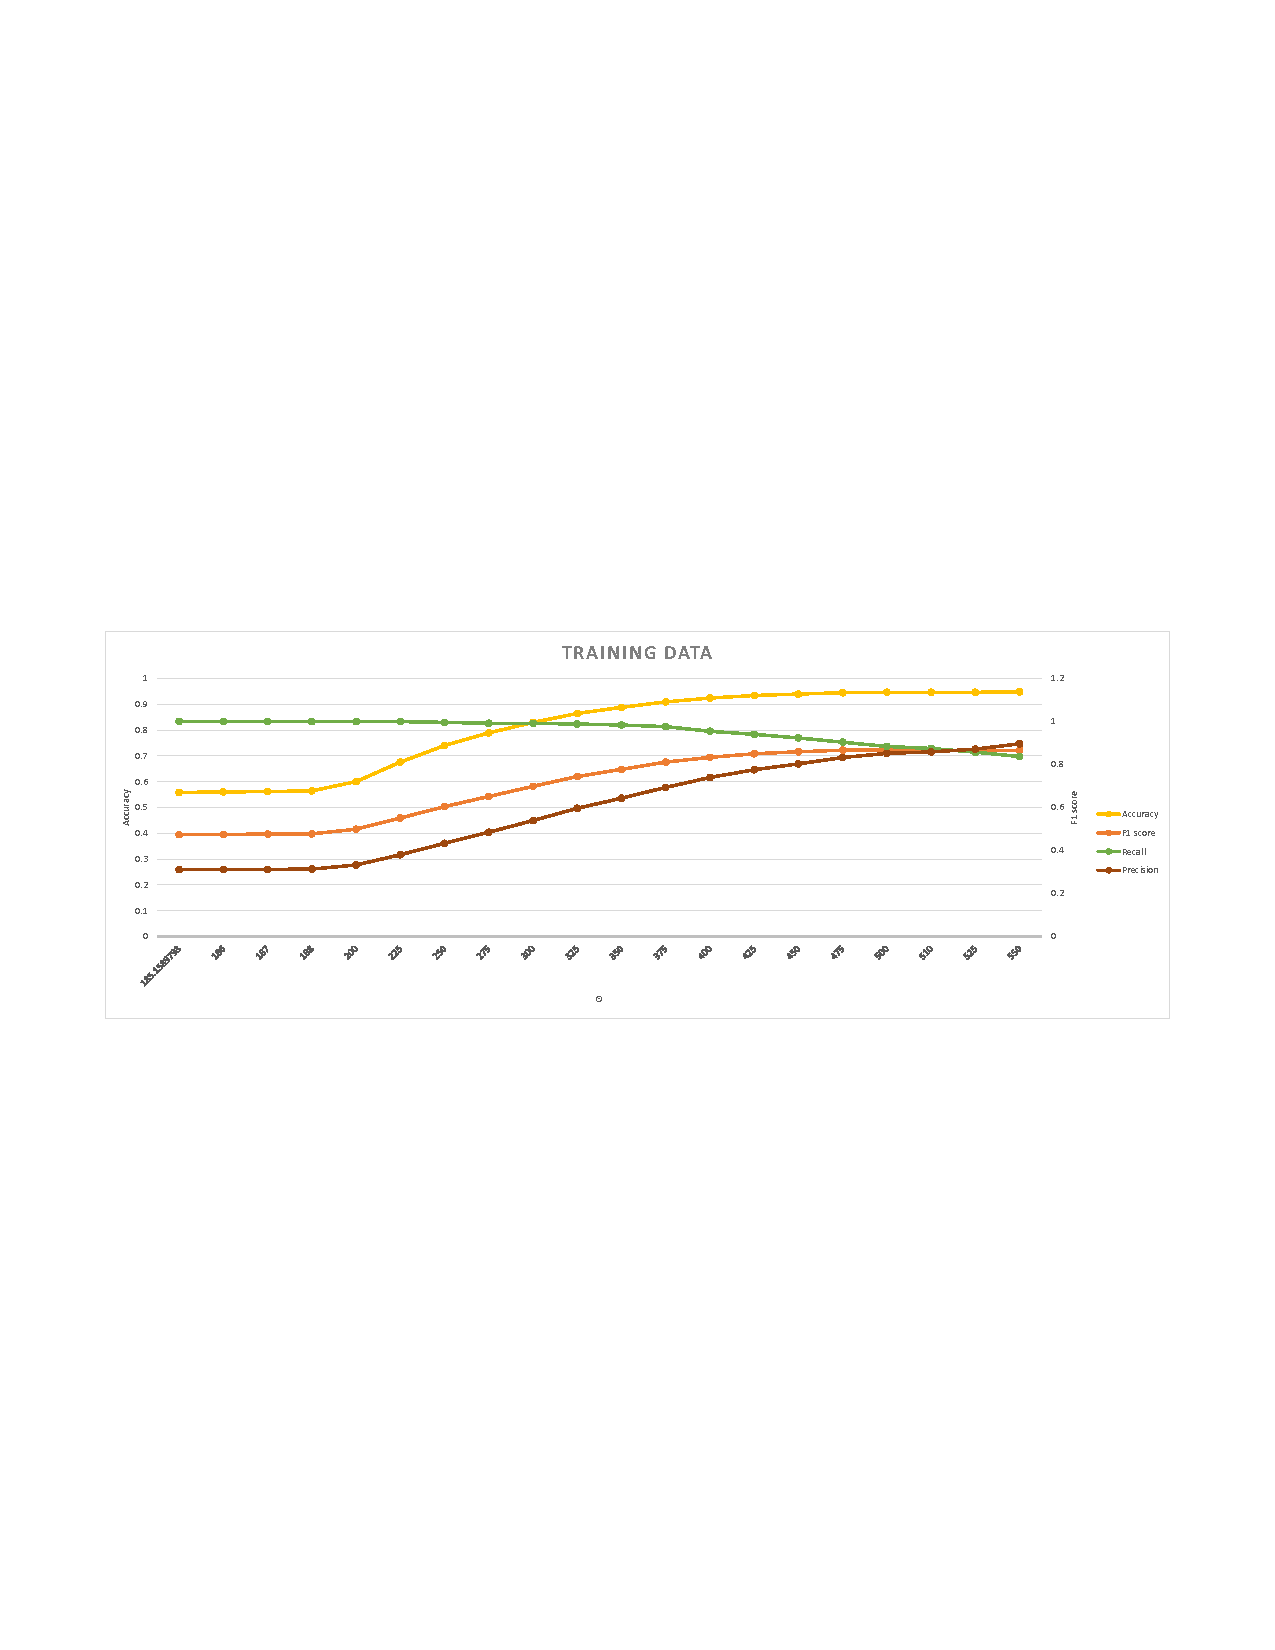
\includegraphics[width=\textwidth]{figs/Edge_Training_Results.pdf}
      \caption[]%
      {The edge analytics training phase.}    
      \label{fig:Edge_Training_Results}
  \end{subfigure}
  \hfill
  \begin{subfigure}[b]{0.475\textwidth}  
      \centering 
      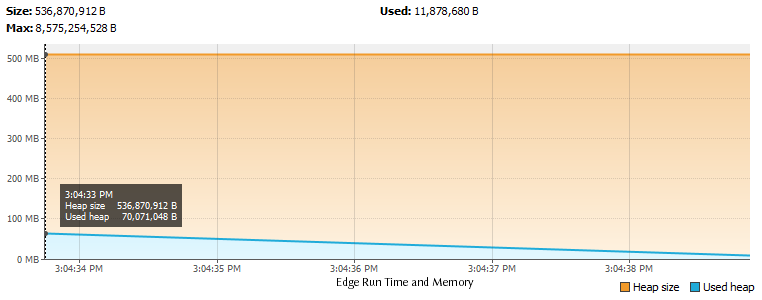
\includegraphics[width=\textwidth]{figs/Edgent_Run_Time_Memory.png}
      \caption[]%
      {The edge layer performance.}    
      \label{fig:Edgent_Run_Time_Memory}
  \end{subfigure}
  \vskip\baselineskip
  \begin{subfigure}[b]{0.475\textwidth}   
      \centering 
      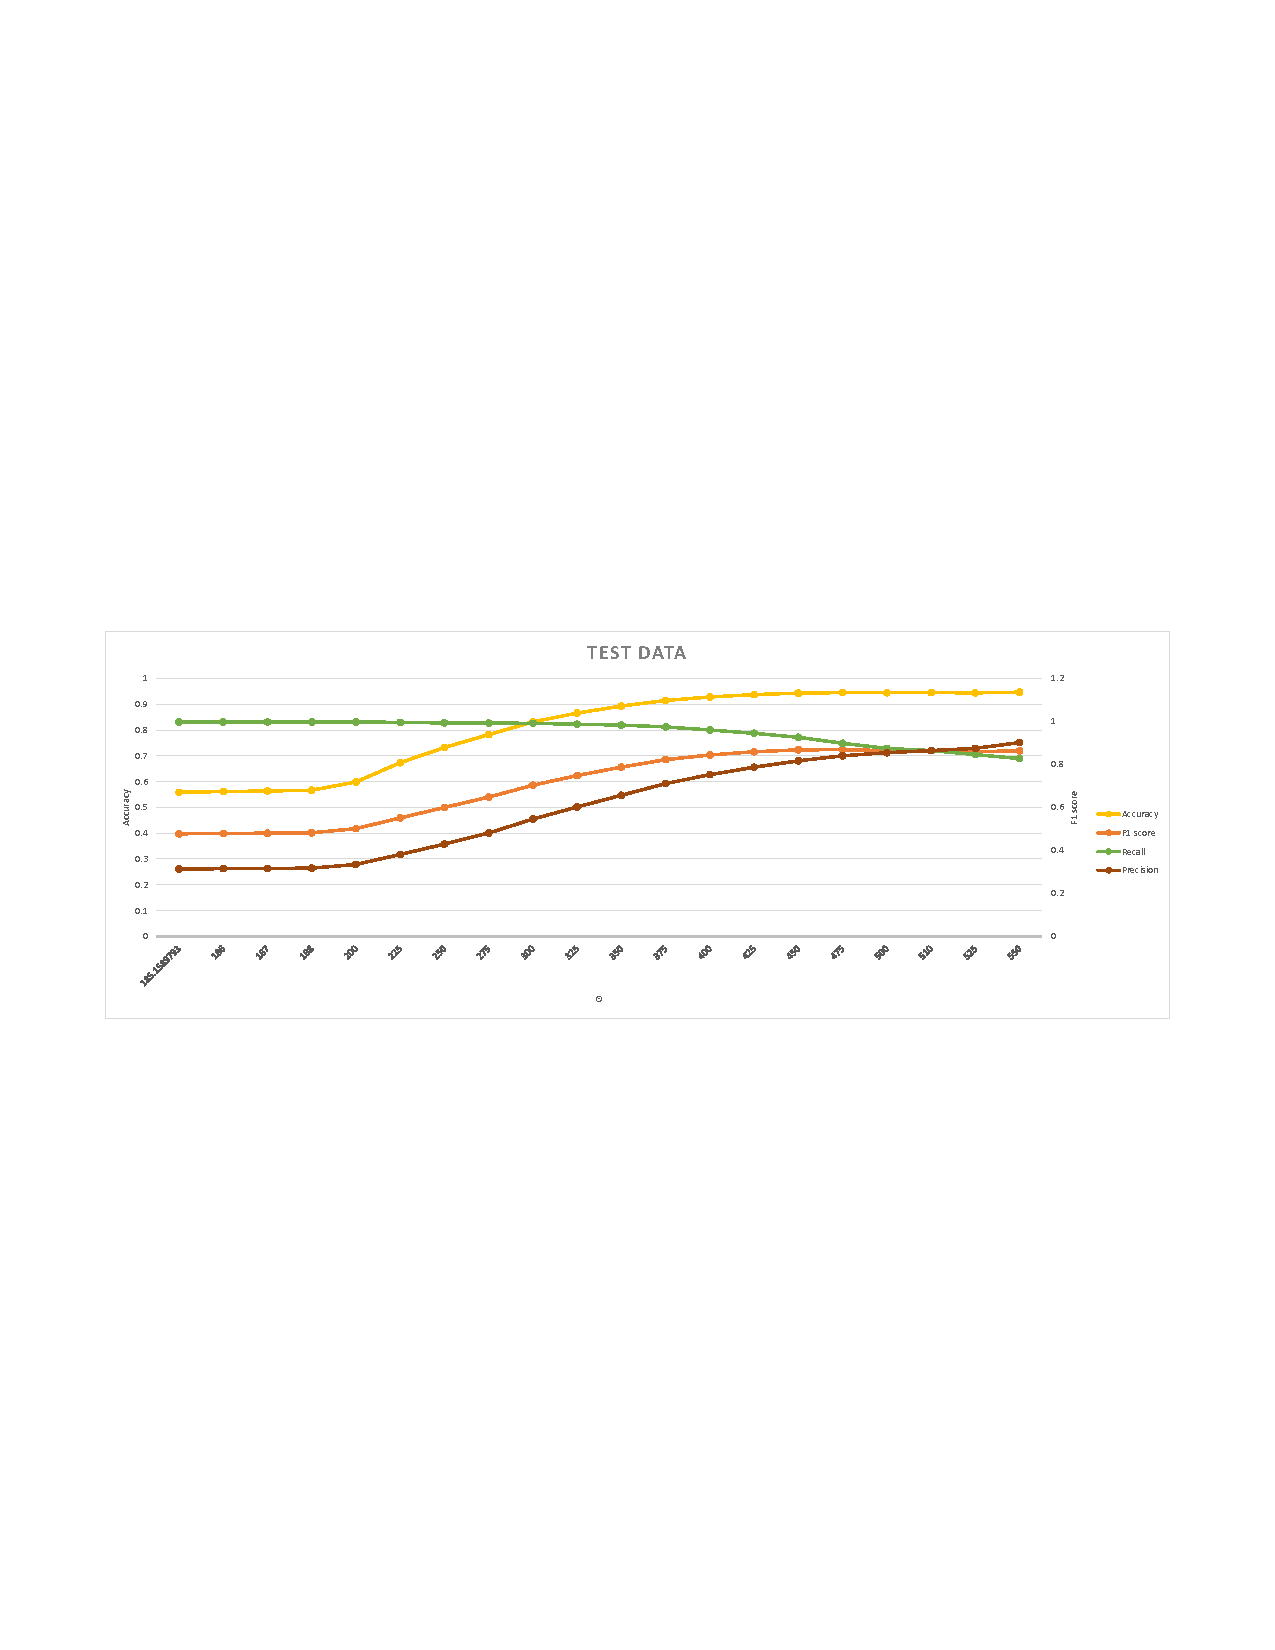
\includegraphics[width=\textwidth]{figs/Edge_Test_Results.pdf}
      \caption[]%
      {The edge analytics training phase.}    
      \label{fig:Edge_Test_Results}
  \end{subfigure}
  \quad
  \begin{subfigure}[b]{0.475\textwidth}   
      \centering 
      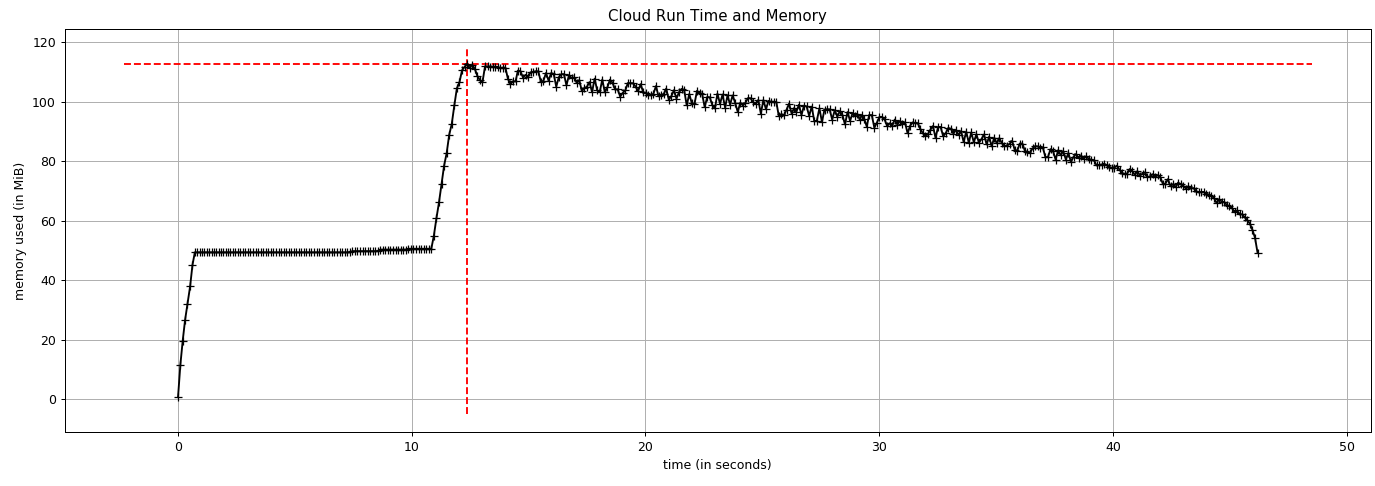
\includegraphics[width=\textwidth]{figs/Cloud_Run_Time_Memory.png}
      \caption[]%
      {The cloud layer performance.}    
      \label{fig:Cloud_Run_Time_Memory}
  \end{subfigure}
  \caption[  ]
  {} 
  \label{fig:compare-edge-training-test-cloud-performance}
\end{figure*}


% \begin{figure}
%   \centering
%   \begin{subfigure}[b]{0.5\textwidth}
%      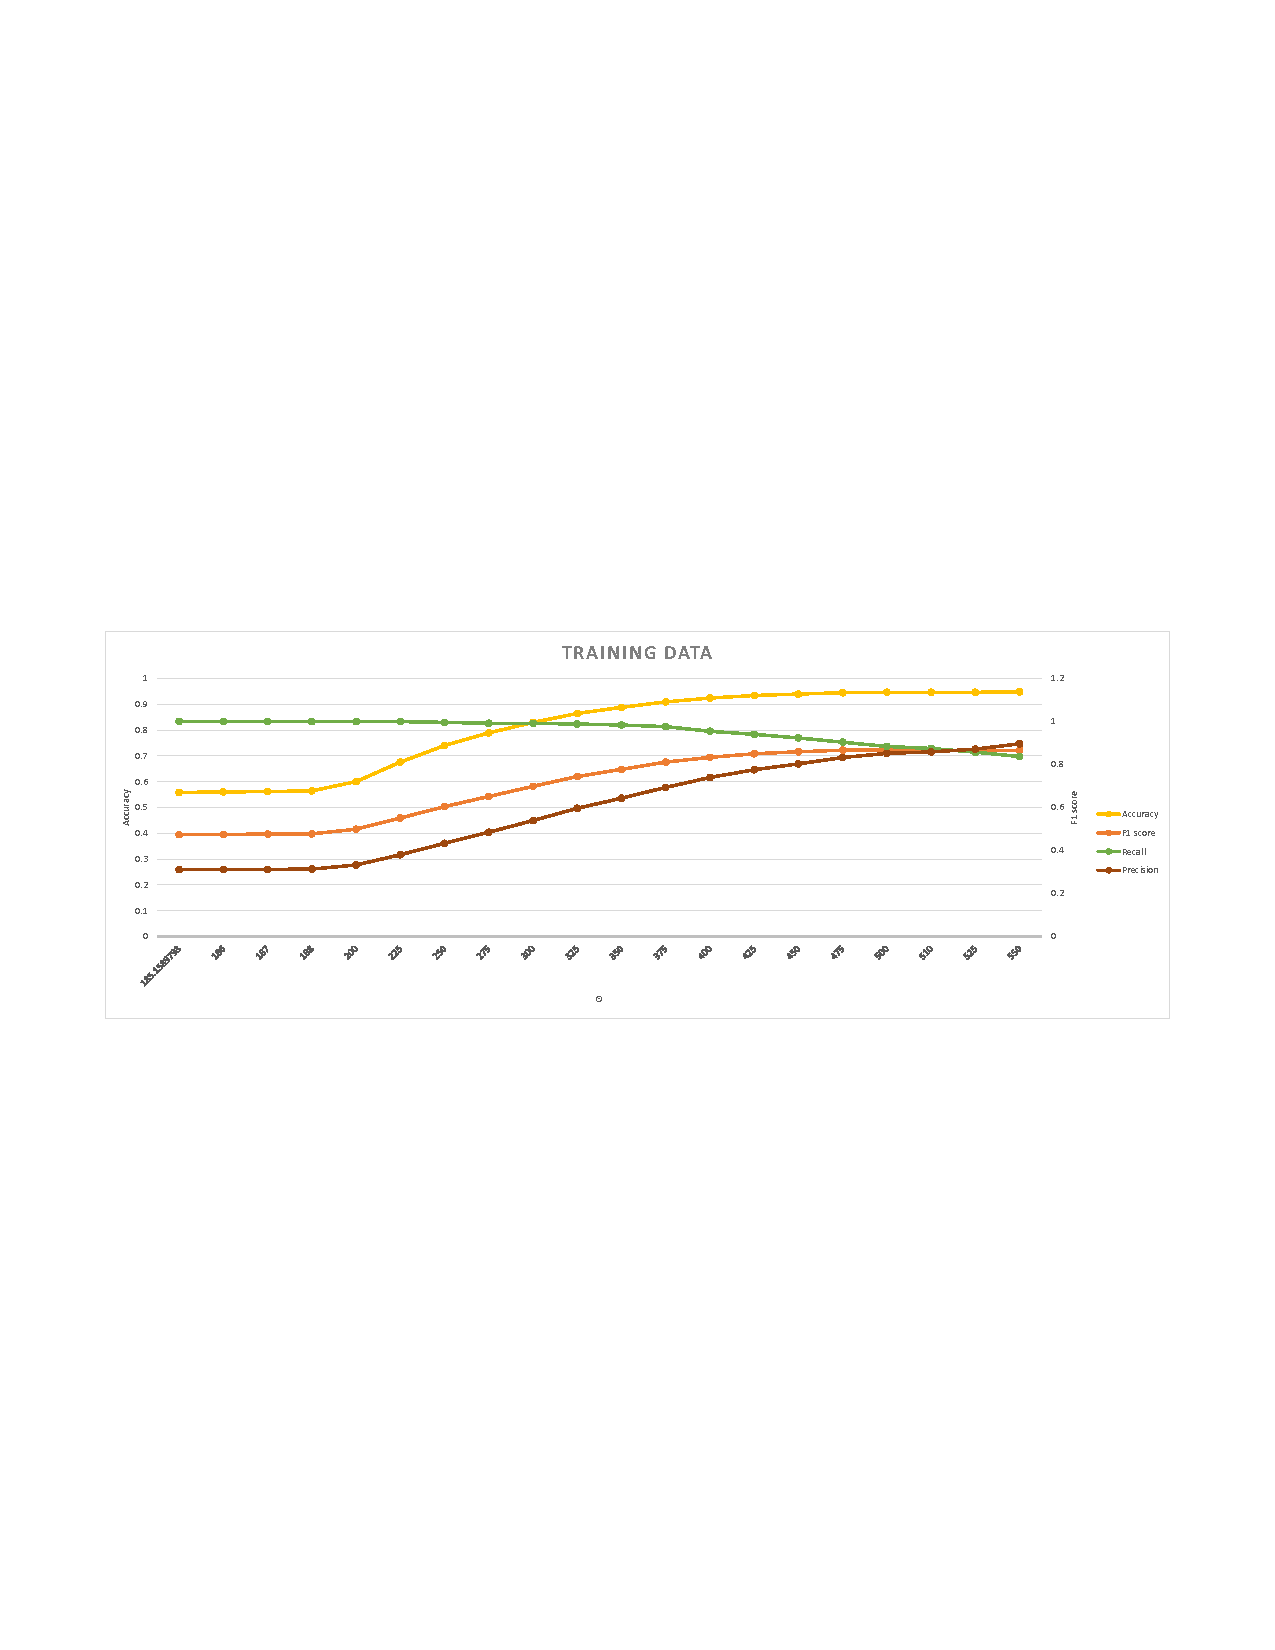
\includegraphics[width=1\textwidth]{figs/Edge_Training_Results.pdf}
%      \caption{}
%      \label{fig:Edge_Training_Results} 
%   \end{subfigure}
  
%   \begin{subfigure}[b]{0.5\textwidth}
%      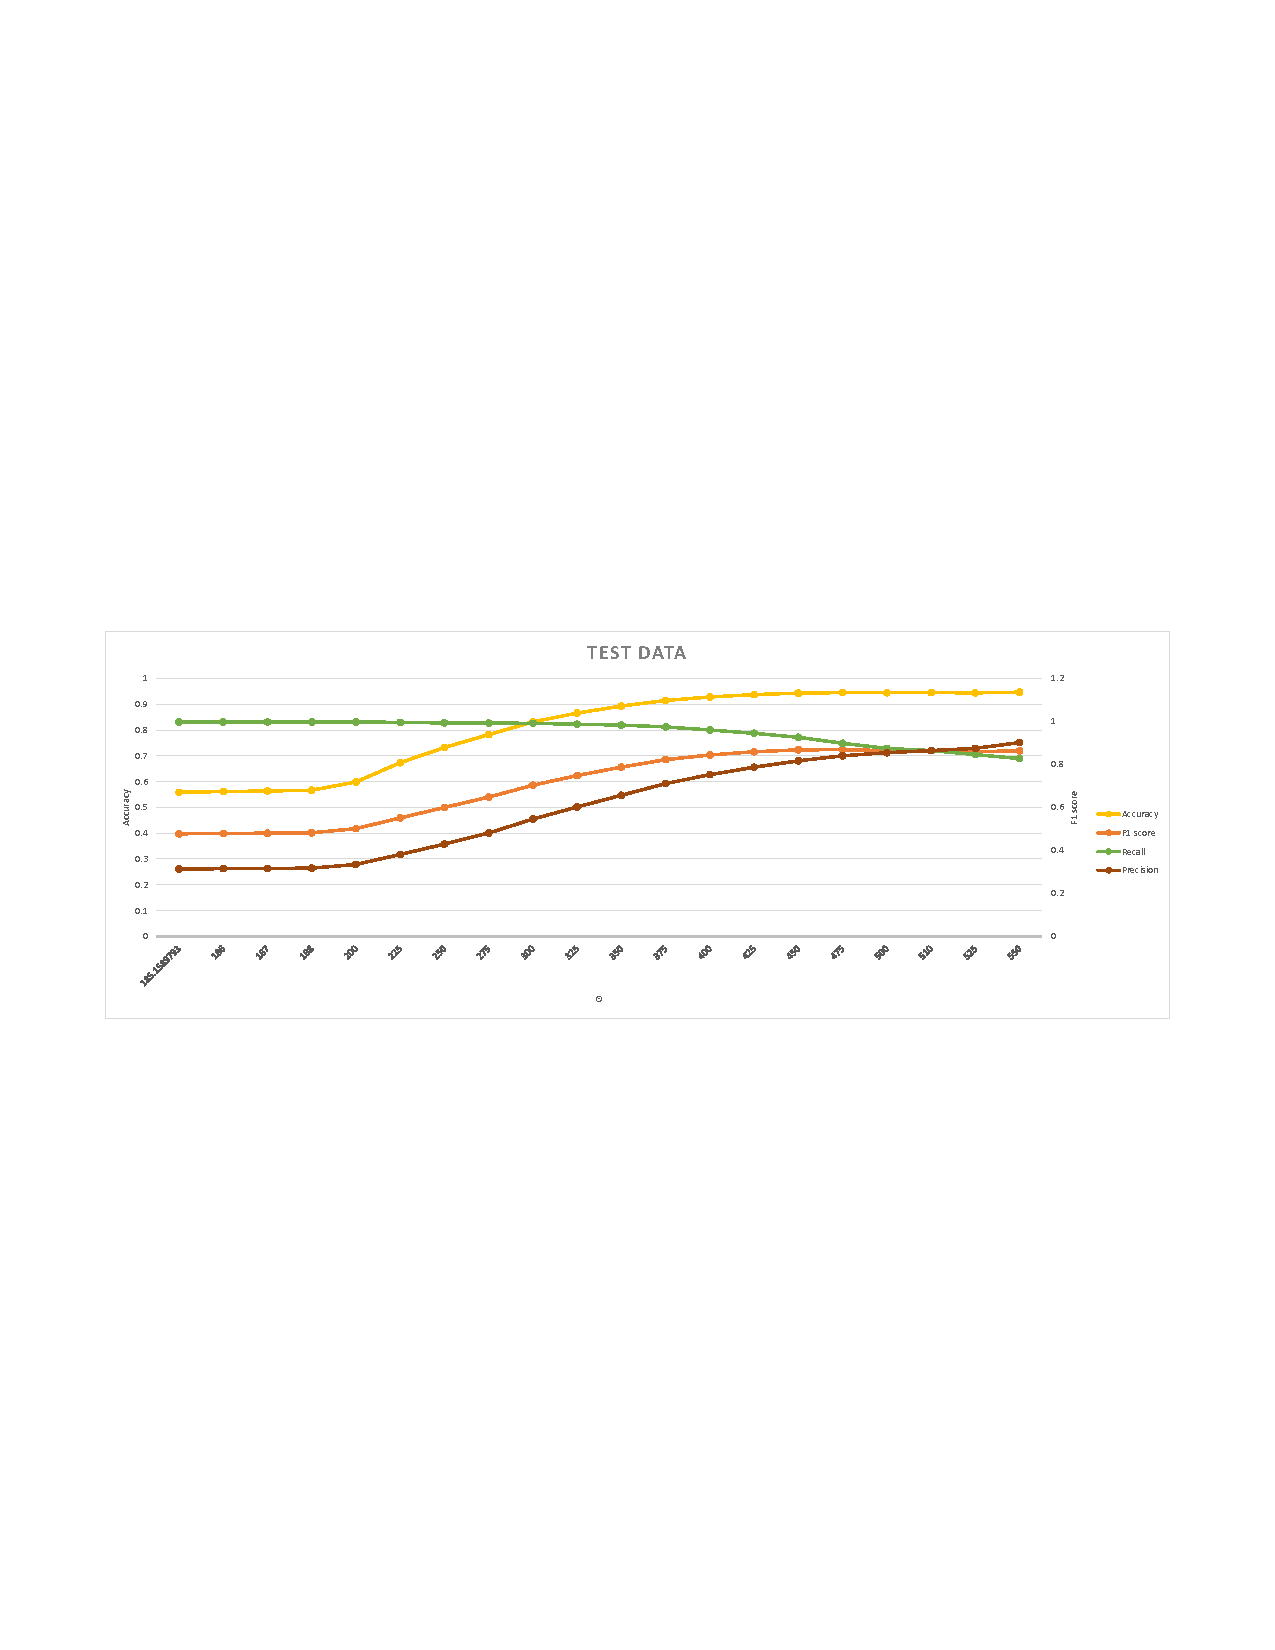
\includegraphics[width=1\textwidth]{figs/Edge_Test_Results.pdf}
%      \caption{}
%      \label{fig:Edge_Test_Results}
%   \end{subfigure}
  
%   \caption[The edge layer analytics results]{(a) The training phase. (b) The test phase.}
% \end{figure}

In this section, we demonstrate the results from the analytics of the two layers presented in the previous section, and then compare the performance of the two. The experiments were performed on a PC with a \fslining{Intel Xeon CPU E3-1271 v3 @ 3.6GHz, and 32GB of memory}.

The accuracy, recall, precision, and F1 score for training and test sets for the edge analytics are shown in figures \ref{fig:Edge_Training_Results} and \ref{fig:Edge_Test_Results}, respectively. Based on the training results, we selected a value of \(\Theta = 300\) as an optimal balance between accuracy and recall, because in such an application we would rather have more false positives (false seizure alarms) than false negatives (missed seizure episodes).

\begin{figure}
  \centering
  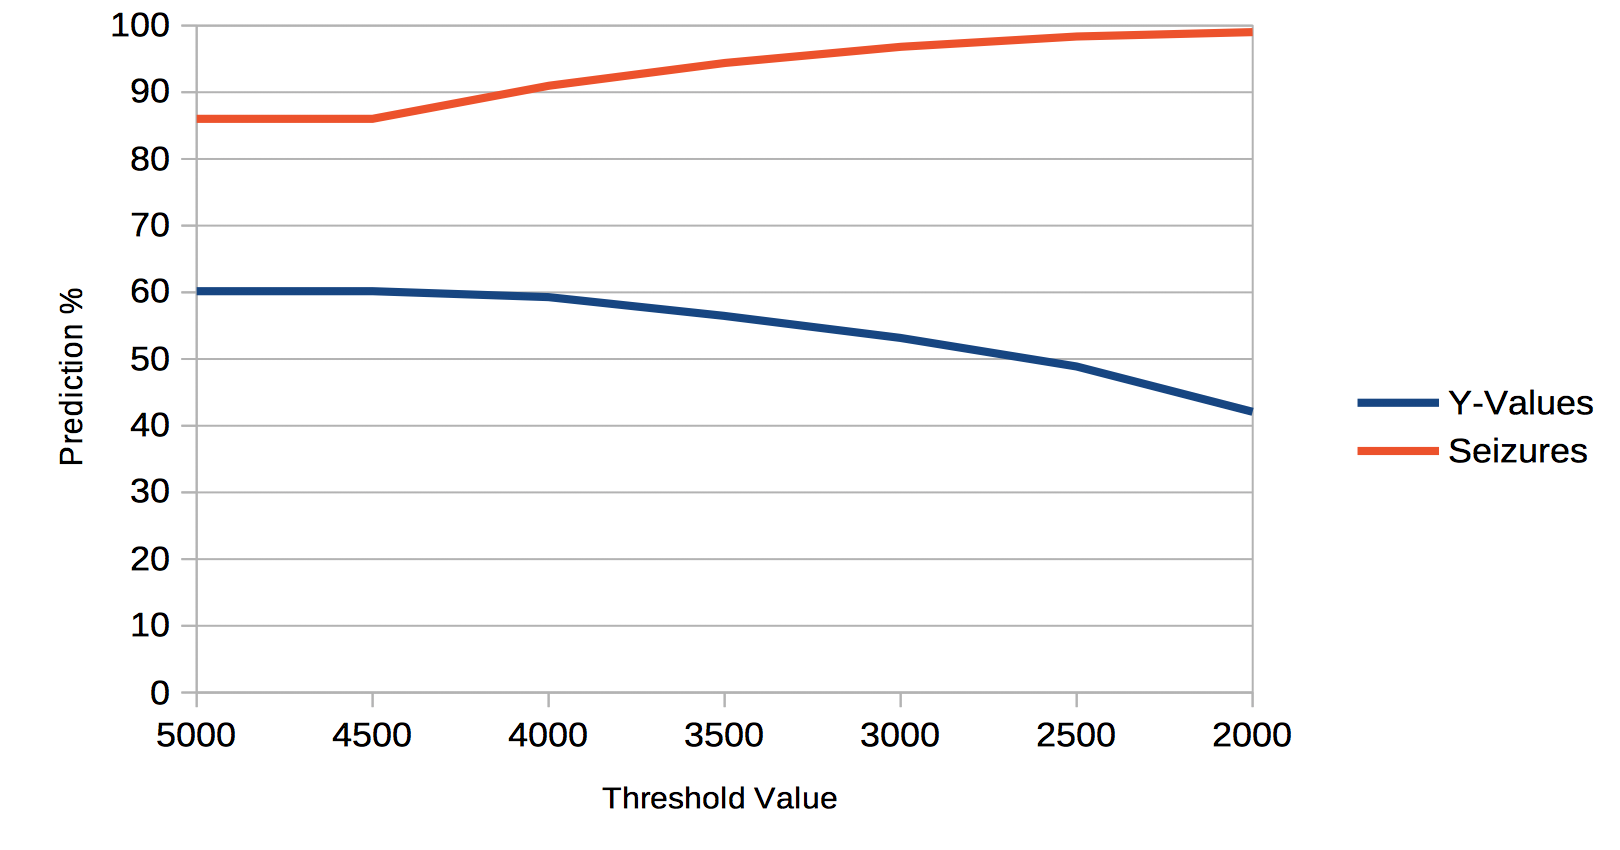
\includegraphics[width=\textwidth]{figs/Threshold.png}
  \caption{The threshold value of the distance measure versus accuracy for the k-means algorithm of the cloud layer.}
  \label{fig.cloud-threshold}
\end{figure}

The threshold value (\(\Theta = 300\)) of the distance measure (\(\mathcal{S}\)) in the k-means algorithm of the cloud layer versus accuracy for test data is displayed in figure~\ref{fig.cloud-threshold}. The results showed that we could achieve higher levels of accuracy as we decreased the threshold/cut-off value for \(\mathcal{S}\) which determines assigning the records to clusters in the k-means algorithm. We selected \(3500\) as an optimal value based on the results of the training phase.

The runtime and memory consumption of the edge and cloud layers for a sample run are shown on figures \ref{fig:Edgent_Run_Time_Memory} and \ref{fig:Cloud_Run_Time_Memory}, respectively. The results show that the edge analytics consumes less memory (almost as half), and performs much faster (about \(2s\) against about \(45s\)).

\section{Discussion}

The results from the Results section demonstrate the advantages of FC for applications which demand near real-time response times, such as those in healthcare.

Instead of having to deal with high accuracy but low latency, as is common on a conventional two-tier IoT/Cloud architecture, an FC architecture --- such as one implemented in this project --- allows us to come up with a balanced tradeoff between performance, latency, and accuracy. Our edge layer analytics solution has lower accuracy in the experiments (\(\approx80\%\)), but it consumes much less resources than the cloud analytics solution, and achieves negligible latency. The cloud solution, on the other hand, achieves higher accuracy (\(\approx95\%\)), but consumes more resources, and incurs a higher response time, considering it will be run in the cloud, farther from the sensors. That means, for example, an application implemented using this architecture can use the edge layer to perform fast though inaccurate analytics for early notification of an onset of epileptic seizures, and at the same time send the data (or an aggregated collection of data) to the cloud for more accurate, but slower, results. Therefore, we believe that we have achieved the desired goal for the project, which is a simple demonstration of obtaining the ability to select from two levels of tradeoffs, as mentioned above, via an architecture of FC.

% todo challenges
During the course of the project, we faced certain challenges, some of which led us to make choices or forgo others stated in our proposal. For example, we planned to implement a light version of k-means or \textsc{dbscan} to analyze the streams; however, as the Apache Edgent is still incubating and lacks a complete documentation, setting it up consumed more time than expected. Moreover, we planned to set up the cloud instance on an IBM Watson IoT hub, and connect the Edgent to its API to send the streams directly to the cloud. This also became unrealistically difficult, because we learned that we needed to write an extra application besides the one in Apache Spark so that it would run in the IBM Streaming Analytics engine.
% todo limitations and future work

We believe that our work can take advantage of many improvements in the future. The first step is to take advantage of a publish-subscribe message broker, such as Apache Kafka or IBM Watson IoT Hub, to process the incoming streams of multiple sensors (or those processed by an edge node), and interact with the cloud. We would also like to try more advanced analytics solutions on the edge; however, the performance requirements of such algorithms and models must be studied and experimented to make them feasible to perform on the edge. Another step would be to receive the result of the analysis from the cloud, and actuate or act based on it on the edge or even the sensors. In the case of our healthcare application, for example, this could be a notification of the final verdict of the cloud on the early detection of a seizure. The cloud layer can also benefit from improvements. Other variants of k-means or other clustering methods could be compared based on accuracy and performance. While the lower response time of the cloud analytics is acceptable, faster responses are still more favorable in order to achieve higher user satisfaction.

% We selected a value of \(\Theta=300\) as a optimal value which best describes the tradeoff between accuracy, recall
%  \clearpage
\bibliographystyle{plain}
{\footnotesize \bibliography{refs}}

\end{document}